Ebben a fejezetben bemutatom a \foreignlanguage{british}{Helpdesk} alkalmazás felé megfogalmazott üzleti igényeket.



\section{Funkcionális igények}

\subsection{E-mail fogadása és küldése}\label{sec:email_fogadas_kuldes}
Az ügyfelektől érkező e-maileket az alkalmazás képes fogadni, hosszú távra megőrizni. Számukra formázott válasz e-mail küldhető.

A rendszernek képesnek kell lennie több e-mail cím kezelésére. A beérkező új üzeneteket a címzettnek megfelelő előre definiált sorhoz kell hozzárendelni.



\subsection{E-mail szálak kezelése}
A rendszer által kezelt üzenetek szálakba rendezve érhetőek el. Egy szál az ügyfél és a felhasználó közötti üzenetváltásokból épül fel.

Az üzenetszálakra vonatkozó összes adat historikusan lekérdezhető, státuszuk \aref{fig:statusz_diagram} ábrán definiált útvonalaknak megfelelően változtatható.  

\begin{figure}[hbt] 
	\centering
	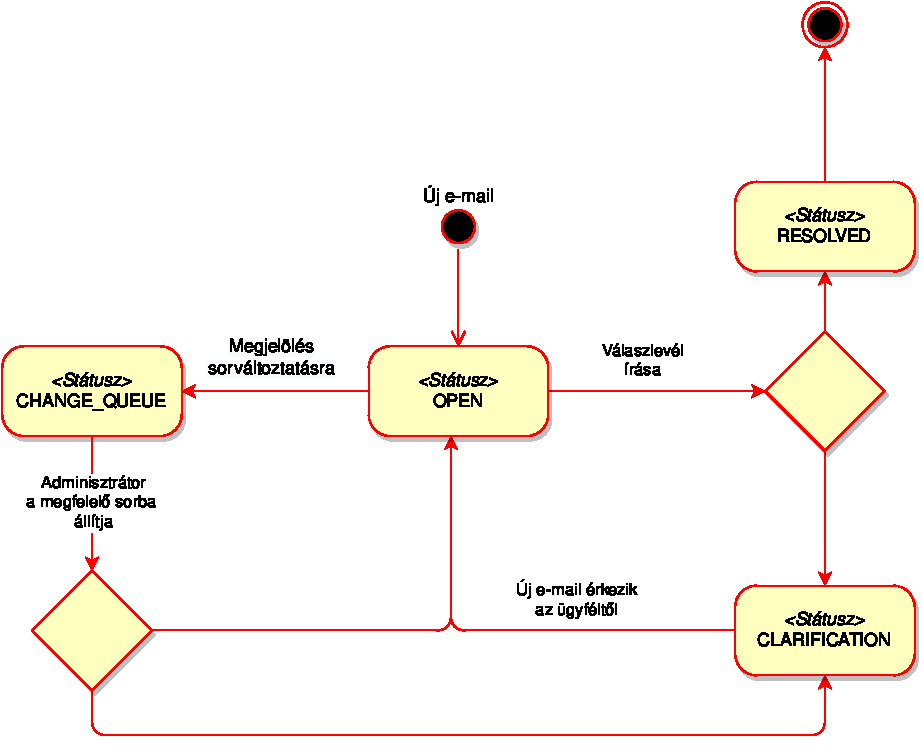
\includegraphics[width=0.85\textwidth]{statusz_diagram_drawio.pdf}
	\caption{Az e-mailszálak státuszváltozásai}
	\label{fig:statusz_diagram}
	\floatfoot{Forrás: saját ábra}
\end{figure}



\subsection{Több felhasználó}\label{sec:tobb_felhasznalo}
A rendszert egyszerre több felhasználó használhatja. Minden felhasználó csak a saját emailszálait kezelheti, csak azokra válaszolhat.

	
Minden felhasználó pontosan egy \aref{sec:email_fogadas_kuldes} fejezetben említett sorhoz tartozik. Csak az ugyanabba a sorba tartozó e-mail szál rendelhető hozzá.
A számára kijelölt szálakat képes -- a saját során belül --  más felhasználóhoz rendelni. 

A felhasználók eltérő jogkörökkel rendelkezhetnek. Az adminisztratív jogkörrel rendelkező felhasználó végzi az új emailszál felhasználóhoz rendelését, valamint a \foreignlanguage{british}{\textit{change queue}} státuszban (\ref{fig:statusz_diagram} ábra) lévő üzenetszálak új sorba irányítását.

A konfigurációs jogkörrel rendelkező felhasználó feladata más felhasználók regisztrálása, valamint az alkalmazásban használt jogkörök (\foreignlanguage{british}{\textit{role}}-ok) kezelése. Lehetősége van továbbá autentikációs események megtekintésére, jelszó visszaállítására és más felhasználók megszemélyesítésére (\foreignlanguage{british}{\textit{impersonate}}).

A felhasználói felületen elérhető funkciókat \aref{fig:funkcio_diagram} ábra foglalja össze.

\begin{figure}[hbt] 
	\centering
	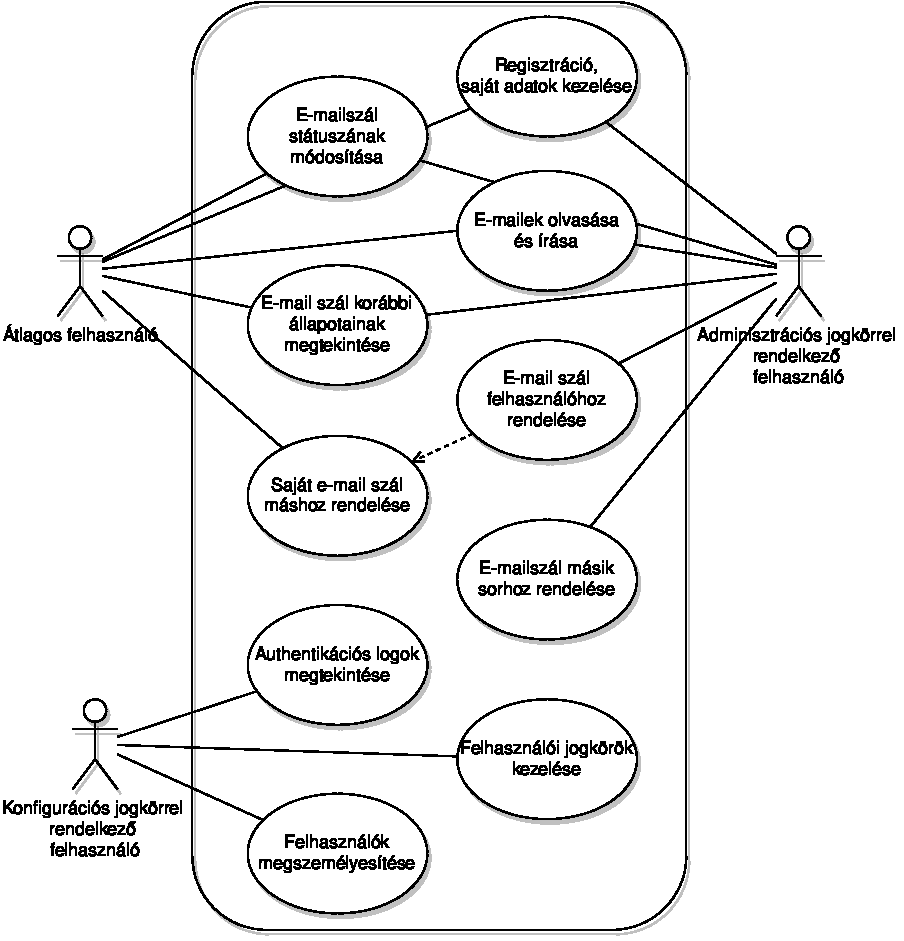
\includegraphics[width=0.85\textwidth]{funkcio_diagram_drawio.pdf}
	\caption[Elérhető funkciók]{Elérhető funkciók jogosultság szerint csoportosítva}
	\label{fig:funkcio_diagram}
	\floatfoot{Forrás: saját ábra}
\end{figure}

\pagebreak
\section{Nem funkcionális igények}	


\subsection[Skálázhatóság]{Horizontális skálázhatóság}
A kiszolgálandó kliensek száma napi és havi szinten is eltérő. Az év egyes időszakaiban nagyobb volumenű ügyfél-interakció prognosztizálható. A hibatűrés javítása, és a megnövekedett forgalom érdekében -- ezekben az előre meghatározott időszakokban --  horizontális skálázódás szükséges.


\subsection{Granuláris felosztottság}\label{sec:granularitas}
A \foreignlanguage{british}{helpdesk} alkalmazást használó ügyfélszolgálat munkaórákban a legaktívabb, míg az e-maileket küldő ügyfelek hétvégente és hétköznap munkaórákon kívül a legaktívabbak.

A hosszútávú tervekben szerepel a \foreignlanguage{british}{helpdesk} alkalmazás és a belső céges levelezés integrálása.

A fenti két szempont miatt célszerű a megvalósítandó funkciók minél nagyobb mértékű szeparálására törekedni.


\subsection{Mérhető indikátorok}\label{sec:indikatorok}
A rendszernek átlagosan $100$ felhasználót kell kiszolgálnia másodpercenként. A várható csúcsteljesítmény $5~000$--$10~000$ lekérdezés másodpercenként. A felhasználók száméra elfogadható legnagyobb válaszidő 3 másodperc/lekérés.


\subsection[L10N]{L10N\footnote{A nyelvi lokalizációt, vagy kulturális beágyazást szokás L10N-ként rövidíteni.}}
A felhasználói, adminisztratív és karbantartói felületek angol nyelven érhetőek el. Több nyelv kezelése nem szükséges.
